\section{极小极大优化}
\label{sec:opt-mmb-minimax}

多目标问题中，各指标的地位平等，只是需要取舍。另一类问题里，两组变量的利益正好相反：一方要使某个量变小，另一方要使它变大。训练一个对输入扰动稳健的模型时，参数要使损失小，而扰动在允许范围内专挑使损失最大的方向。这时目标值取决于双方的选择次序，本节先把次序和值说清楚，再给出检验一对候选的证书，最后比较两种迭代方法在同一个简单问题上的行为。

本节考虑
\begin{equation}
\label{eq:opt-mmb-minimax}
\min_{\bm x\in X}\ \max_{\bm y\in Y}\ \phi(\bm x,\bm y),
\end{equation}
称为\term{极小极大问题}（minimax problem），其中$X\subseteq\mathbb R^{d}$、$Y\subseteq\mathbb R^{q}$非空，$\phi:X\times Y\to\mathbb R$。$\bm x$是最小化方的变量，$\bm y$是最大化方的变量。

\subsection{响应顺序与最坏值}
\label{sec:opt-mmb-order}

\paragraph{一个猜数游戏}
先看一个一维例子。我们选一个数$x\in\mathbb R$，对手在看到$x$之后从$[-1,1]$中选一个数$y$，我们付出损失$\phi(x,y)=(x-y)^2$。对手看到$x$后会把$y$放到离$x$最远的端点，于是$x$的实际损失是
\[
\bar\phi(x)=\max_{|y|\leq1}(x-y)^2=(|x|+1)^2.
\]
我们应当选$x=0$，最坏损失为$1$。若次序反过来，对手先公布$y$、我们再选$x$，我们只需令$x=y$，损失为零。同一个函数，先选还是后选，得到的值相差$1$。图~\ref{fig:opt-mmb-worst-case}画出了几条$(x-y)^2$及其上包络$\bar\phi$：极小极大问题最小化的是这条上包络，而不是其中任何一条曲线。

\begin{figure}[!htbp]
  \centering
  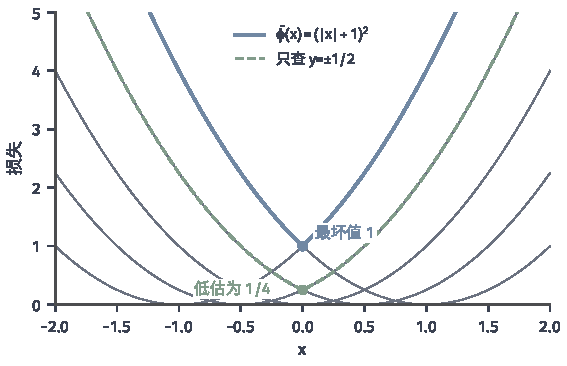
\includegraphics[width=96mm]{figures/03-optimization-evolution-and-signals/01-optimization/matplotlib/c7-worst-case-envelope/figure.pdf}
  \caption{猜数游戏$\phi(x,y)=(x-y)^2$，$y\in[-1,1]$。灰线是$y\in\{0,\pm\frac12,\pm1\}$时的$(x-y)^2$，蓝色粗线是对全部$y\in[-1,1]$取最大的上包络$\bar\phi(x)=(|x|+1)^2$，其最小值$1$在$x=0$处达到。绿色虚线是只检查$y=\pm\frac12$时的包络$(|x|+\frac12)^2$，它把$x=0$的最坏值低估为$1/4$。}
  \label{fig:opt-mmb-worst-case}
\end{figure}

\paragraph{外层值函数}
一般地，问题~\eqref{eq:opt-mmb-minimax}的次序是：外层先选$\bm x$，内层看到$\bm x$后选$\bm y$。外层面对的是值函数
\begin{equation}
\label{eq:opt-mmb-upper-value-function}
\bar\phi(\bm x)=\sup_{\bm y\in Y}\phi(\bm x,\bm y),
\end{equation}
问题~\eqref{eq:opt-mmb-minimax}就是在$X$上最小化$\bar\phi$，其最优值$\overline v=\inf_{\bm x\in X}\bar\phi(\bm x)$称为上值。对称地，定义$\underline\phi(\bm y)=\inf_{\bm x\in X}\phi(\bm x,\bm y)$与下值$\underline v=\sup_{\bm y\in Y}\underline\phi(\bm y)$，它对应内层先选的次序。要让上确界~\eqref{eq:opt-mmb-upper-value-function}确实被某个$\bm y$达到，可以要求$Y$紧且$\phi(\bm x,\cdot)$连续，这正是第~\ref{chap:optimization}章的存在性条件用在内层上。猜数游戏中$Y=[-1,1]$紧，最大值在端点达到。

\begin{lemma}[弱极小极大不等式]
\label{lem:opt-mmb-weak-minimax}
对任意$\phi$与非空的$X,Y$，有$\underline\phi(\bm y)\leq\phi(\bm x,\bm y)\leq\bar\phi(\bm x)$对所有$\bm x\in X,\bm y\in Y$成立，因而$\underline v\leq\overline v$。
\end{lemma}

\begin{proof}
左右两个不等式分别来自下确界与上确界的定义。于是任意$\bm x,\bm y$都满足$\underline\phi(\bm y)\leq\bar\phi(\bm x)$；先对$\bm y$取上确界，再对$\bm x$取下确界即得$\underline v\leq\overline v$。
\end{proof}

不等式说明后选的一方总不吃亏，能看到对方选择的一方至少能做到与先选时一样好。猜数游戏中$\underline v=0<1=\overline v$，等号不成立。

\paragraph{近似内层给出的是下界}
实际计算中，内层的最大化往往只能近似完成。若只在一个子集$Y'\subseteq Y$中搜索，或者内层算法停在某个$\tilde{\bm y}$，所得的$\max_{\bm y\in Y'}\phi(\bm x,\bm y)$或$\phi(\bm x,\tilde{\bm y})$都不超过$\bar\phi(\bm x)$。它们是真实最坏值的下界，而不是外层目标的值。图~\ref{fig:opt-mmb-worst-case}中只检查$y=\pm\frac12$时，$x=0$的最坏损失被报告为$1/4$，而真实值是$1$。若外层据此宣称“最坏损失已降到$1/4$”，结论是错的。要把近似值当作外层目标使用，需要另外控制内层误差，例如内层是凹最大化时用第~\ref{chap:constrained-optimization}章的对偶界给出上界。

允许集合本身也是问题的一部分。把猜数游戏中的$Y$换成$[-\rho,\rho]$，上包络变成$(|x|+\rho)^2$，最坏值变成$\rho^2$。比较两种稳健训练算法之前，必须先确认它们面对的是同一个扰动集合，否则比较的是两个不同的问题。

\subsection{鞍点、间隙与最值交换}
\label{sec:opt-mmb-saddle-gap}

一个候选$\bm x$的好坏由$\bar\phi(\bm x)$决定，而计算$\bar\phi$需要解一个内层最大化。若同时手握一个$\bm y$，能否用一对候选互相印证？答案是比较两个次序下的值。

\begin{definition}[极小极大鞍点]
\label{def:opt-mmb-saddle}
若$(\bm x^\star,\bm y^\star)\in X\times Y$满足
\[
\phi(\bm x^\star,\bm y)\leq\phi(\bm x^\star,\bm y^\star)\leq\phi(\bm x,\bm y^\star)\qquad\text{对所有}\ \bm x\in X,\ \bm y\in Y,
\]
称它为$\phi$在$X\times Y$上的\term{极小极大鞍点}（minimax saddle point）。
\end{definition}

鞍点的含义是双方互为最优响应：固定$\bm y^\star$时，$\bm x^\star$是最小化方的全局最优选择；固定$\bm x^\star$时，$\bm y^\star$是最大化方的全局最优选择。这与多元微积分中由Hessian正负曲率描述的鞍点是两回事。图~\ref{fig:opt-mmb-saddle-surfaces}中两张曲面形状完全相同，都在原点有一个零梯度、Hessian不定的驻点。左图$\phi=x^2-y^2$沿$x$方向向上弯、沿$y$方向向下弯，最小化方$x$与最大化方$y$都在原点取到最优，原点是极小极大鞍点。右图$\phi=y^2-x^2$只是把两个方向的角色交换，此时固定$y=0$，$\phi(x,0)=-x^2$在$x=0$处取最大而非最小，原点不是极小极大鞍点。判断鞍点必须知道哪个变量属于哪一方。

\begin{figure*}[!htbp]
  \centering
  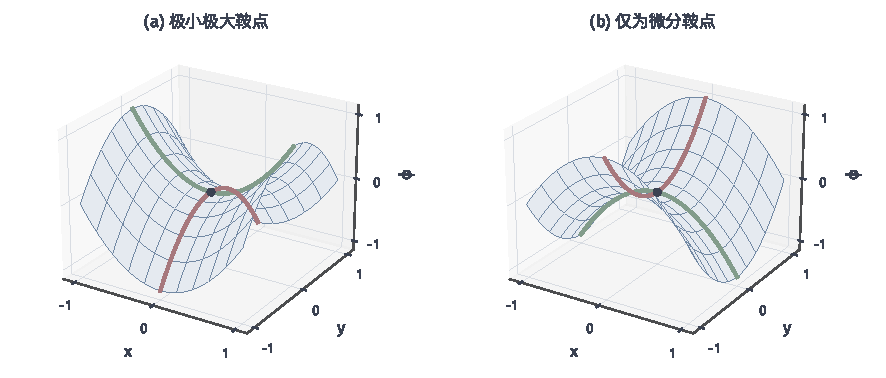
\includegraphics[width=150mm]{figures/03-optimization-evolution-and-signals/01-optimization/matplotlib/c7-saddle-surfaces/figure.pdf}
  \caption{同一形状的马鞍曲面，$x$是最小化方，$y$是最大化方。绿线是$y=0$时沿$x$的截线，红线是$x=0$时沿$y$的截线。(a)$\phi=x^2-y^2$：绿线在原点取最小、红线在原点取最大，原点是极小极大鞍点。(b)$\phi=y^2-x^2$：截线方向反了，原点只是Hessian不定的驻点，最小化方离开原点反而有利。}
  \label{fig:opt-mmb-saddle-surfaces}
\end{figure*}

\paragraph{原始--对偶间隙}
对一对候选$(\bm x,\bm y)$，定义
\begin{equation}
\label{eq:opt-mmb-gap}
\operatorname{gap}(\bm x,\bm y)=\bar\phi(\bm x)-\underline\phi(\bm y),
\end{equation}
称为\term{原始--对偶间隙}（primal--dual gap）。由引理~\ref{lem:opt-mmb-weak-minimax}它总是非负的。

\begin{lemma}[间隙作为证书]
\label{lem:opt-mmb-gap-certificate}
设$\bar\phi(\bm x)$与$\underline\phi(\bm y)$有限。则$\operatorname{gap}(\bm x,\bm y)=0$当且仅当$(\bm x,\bm y)$是极小极大鞍点。此外总有$\bar\phi(\bm x)-\overline v\leq\operatorname{gap}(\bm x,\bm y)$与$\underline v-\underline\phi(\bm y)\leq\operatorname{gap}(\bm x,\bm y)$。
\end{lemma}

\begin{proof}
若$(\bm x,\bm y)$是鞍点，定义中的不等式对所有$\bm x',\bm y'$成立，取上确界与下确界得$\bar\phi(\bm x)\leq\phi(\bm x,\bm y)\leq\underline\phi(\bm y)$，结合非负性得间隙为零。反过来，若$\bar\phi(\bm x)=\underline\phi(\bm y)$，由$\underline\phi(\bm y)\leq\phi(\bm x,\bm y)\leq\bar\phi(\bm x)$知三者相等，于是对所有$\bm x',\bm y'$有$\phi(\bm x,\bm y')\leq\bar\phi(\bm x)=\phi(\bm x,\bm y)=\underline\phi(\bm y)\leq\phi(\bm x',\bm y)$。最后两个不等式由$\underline\phi(\bm y)\leq\underline v\leq\overline v$得到。
\end{proof}

间隙的意义在于它把一个需要“对所有$\bm x',\bm y'$检查”的定义，变成两个最优响应问题的数值：算出$\bar\phi(\bm x)$与$\underline\phi(\bm y)$，相减即可知道$\bm x$离最优上值至多差多少。代价是要能精确求出两侧的最优响应，或至少给出$\bar\phi(\bm x)$的上界与$\underline\phi(\bm y)$的下界。

\paragraph{双线性盒例}
取$X=Y=[-1,1]$，$\phi(x,y)=xy$。固定$x$时$xy$关于$y$线性，最大值在端点，$\bar\phi(x)=|x|$；同理$\underline\phi(y)=-|y|$。于是$\overline v=\underline v=0$，$\operatorname{gap}(x,y)=|x|+|y|$，唯一鞍点是原点。这个例子在后两小节反复使用：它简单到可以手算，却已经足以让最直接的算法失败。

\paragraph{凸凹条件下的最值交换}
猜数游戏中上值严格大于下值，鞍点不存在。什么条件下两个次序给出同一个值？关键是凸凹结构。

\begin{theorem}[紧凸凹条件下的极小极大定理]
\label{thm:opt-mmb-minimax}
设$X,Y$非空、紧、凸，$\phi$在$X\times Y$上连续，对每个$\bm y\in Y$，$\phi(\cdot,\bm y)$在$X$上凸；对每个$\bm x\in X$，$\phi(\bm x,\cdot)$在$Y$上凹。则
\[
\min_{\bm x\in X}\max_{\bm y\in Y}\phi(\bm x,\bm y)=\max_{\bm y\in Y}\min_{\bm x\in X}\phi(\bm x,\bm y),
\]
两侧的最值都能达到，且存在极小极大鞍点。
\end{theorem}

\begin{proof}
由引理~\ref{lem:opt-mmb-weak-minimax}，只需证$\underline v\geq\overline v$。连续函数在紧集上有界，所以$\overline v$有限。任取$c<\overline v$。

第一步，用紧性化为有限个$\bm y$。对每个$\bm x\in X$有$\bar\phi(\bm x)\geq\overline v>c$，故存在$\bm y$使$\phi(\bm x,\bm y)>c$。于是集合$U_{\bm y}=\{\bm x\in X:\phi(\bm x,\bm y)>c\}$覆盖$X$；它们由连续性是$X$中的开集，紧性给出有限个$\bm y_1,\dots,\bm y_k$使每个$\bm x$至少满足一个$\phi(\bm x,\bm y_i)>c$。函数$\bm x\mapsto\max_i\phi(\bm x,\bm y_i)$连续，在紧集$X$上达到最小值，记为$c'$，则$c'>c$。

第二步，用凸性与分离得到权重。令$K=\{\bm z\in\mathbb R^k:\text{存在}\ \bm x\in X\ \text{使}\ z_i\geq\phi(\bm x,\bm y_i)\ \forall i\}$。由$X$凸与每个$\phi(\cdot,\bm y_i)$凸，$K$是凸集。$K$与开凸集$O=\{\bm z:z_i<c'\ \forall i\}$不相交，否则会有$\bm x$使$\max_i\phi(\bm x,\bm y_i)<c'$。为得到分离方向，考虑差集$D=K-O=\{\bm z-\bm w:\bm z\in K,\ \bm w\in O\}$。它是凸集，又因$O$是开集而为开集，且不含原点。第~\ref{chap:constrained-optimization}章由投影证明了点与闭凸集的严格分离；把它用在$D$的闭包上：开凸集的闭包与它有相同的内部，所以原点或者在闭包之外，可以直接严格分离，或者落在闭包的边界上，这时取闭包之外趋于原点的点逐一分离，单位法向量有收敛子列，极限仍是单位向量（与该章强对偶证明中取分离方向极限的做法相同）。两种情形都给出非零$\bm\lambda\in\mathbb R^k$，使$\langle\bm\lambda,\bm z-\bm w\rangle\geq0$，即$\langle\bm\lambda,\bm z\rangle\geq\langle\bm\lambda,\bm w\rangle$对所有$\bm z\in K$、$\bm w\in O$成立。$K$中的点把任一分量增大后仍在$K$中，若某个$\lambda_i<0$，左侧可趋于$-\infty$，矛盾，所以$\bm\lambda\geq\bm 0$，可归一化为$\sum_i\lambda_i=1$。令$\bm w$趋于$(c',\dots,c')$，得$\sum_i\lambda_i\phi(\bm x,\bm y_i)\geq c'$对所有$\bm x\in X$成立。

第三步，用凹性把有限个$\bm y_i$合成一个。令$\bar{\bm y}=\sum_i\lambda_i\bm y_i$，由$Y$凸知$\bar{\bm y}\in Y$；由$\phi(\bm x,\cdot)$凹，$\phi(\bm x,\bar{\bm y})\geq\sum_i\lambda_i\phi(\bm x,\bm y_i)\geq c'$对所有$\bm x$成立。于是$\underline v\geq\underline\phi(\bar{\bm y})\geq c'>c$。由$c<\overline v$的任意性得$\underline v\geq\overline v$。

最后，$\bar\phi$是一族连续函数的上确界，因而下半连续，在紧集$X$上达到最小值；同理$\underline\phi$上半连续，在$Y$上达到最大值。取相应的最优点$\bm x^\star,\bm y^\star$，其间隙为$\overline v-\underline v=0$，由引理~\ref{lem:opt-mmb-gap-certificate}它们构成鞍点。
\end{proof}

证明中每个条件各有职责。紧性与连续性把无穷多个对手选择化为有限个，并保证最值达到；关于$\bm x$的凸性使集合$K$凸，从而能被分离出权重；关于$\bm y$的凹性把“按权重混合几个$\bm y_i$”合成为$Y$中的一个点。猜数游戏缺的正是最后一条：$(x-y)^2$关于$y$是凸的，对手在$y=\pm1$之间的“混合”$\frac12(x+1)^2+\frac12(x-1)^2=x^2+1$不小于$1$，但单点$y=0$只给出$x^2$，混合无法合成为一个纯选择。这一定理是Sion所证更一般结论的特例\cite{sion1958}。

在非凸对抗问题中，例如参数和扰动都经过深度网络的稳健训练，凸凹条件通常不成立，上值与下值可以不同，也无法保证鞍点存在。零梯度也不能代替间隙证书：在$X=Y=[-1,1]$上取$\phi=y^2-x^2$，原点处两个偏梯度都为零，但$\bar\phi(0)=\max_y y^2=1$，$\underline\phi(0)=\min_x(-x^2)=-1$，间隙为$2$。

\subsection{梯度下降—上升}
\label{sec:opt-mmb-gda}

最自然的算法是让双方各按自己的方向走一步：最小化方沿负梯度，最大化方沿正梯度，再各自投影回可行集。设$\phi$在包含$X\times Y$的开集上可微，$X,Y$为非空闭凸集，$\Pi_X,\Pi_Y$是第~\ref{chap:opt-nonsmooth}章的欧氏投影。

\paragraph{同时更新与交替更新}
同时版本中，两个偏梯度都在同一个旧点$(\bm x^{(t)},\bm y^{(t)})$处计算，见算法~\ref{alg:opt-mmb-gda}。交替版本先更新$\bm x$，再在新的$\bm x^{(t+1)}$处计算$\bm y$的梯度：
\[
\begin{aligned}
\bm x^{(t+1)}&=\Pi_X\bigl(\bm x^{(t)}-\eta\nabla_{\bm x}\phi(\bm x^{(t)},\bm y^{(t)})\bigr),\\
\bm y^{(t+1)}&=\Pi_Y\bigl(\bm y^{(t)}+\eta\nabla_{\bm y}\phi(\bm x^{(t+1)},\bm y^{(t)})\bigr).
\end{aligned}
\]
两者的差别只在一个梯度的求值位置，却是不同的迭代，下面会看到它们的轨迹也不同。讨论任何轨迹之前，都要先固定步长、投影规则和更新次序。

\begin{algorithm}[投影同时梯度下降—上升]
\label{alg:opt-mmb-gda}
\begin{algorithmic}[1]
\Require 初始点$\bm x^{(0)}\in X$，$\bm y^{(0)}\in Y$，步长$\eta>0$，迭代次数$T$
\Ensure 迭代点$(\bm x^{(T)},\bm y^{(T)})$，以及可用时的间隙估计
\For{$t=0,1,\dots,T-1$}
  \State 在同一点计算$\bm g_x\gets\nabla_{\bm x}\phi(\bm x^{(t)},\bm y^{(t)})$，$\bm g_y\gets\nabla_{\bm y}\phi(\bm x^{(t)},\bm y^{(t)})$
  \State $\bm x^{(t+1)}\gets\Pi_X(\bm x^{(t)}-\eta\bm g_x)$，$\bm y^{(t+1)}\gets\Pi_Y(\bm y^{(t)}+\eta\bm g_y)$
\EndFor
\end{algorithmic}
\end{algorithm}

\paragraph{双线性问题上的绕圈}
先去掉约束，看$\phi(x,y)=xy$在全平面上的行为。$\nabla_x\phi=y$，$\nabla_y\phi=x$，同时更新为
\[
\begin{pmatrix}x^{(t+1)}\\y^{(t+1)}\end{pmatrix}=\begin{pmatrix}1&-\eta\\ \eta&1\end{pmatrix}\begin{pmatrix}x^{(t)}\\y^{(t)}\end{pmatrix}.
\]
这个矩阵是旋转矩阵乘以$\sqrt{1+\eta^2}$，直接计算得$(x^{(t+1)})^2+(y^{(t+1)})^2=(1+\eta^2)\bigl((x^{(t)})^2+(y^{(t)})^2\bigr)$。每一步都绕鞍点转一个角度并向外放大，任何非零初值都螺旋式地远离鞍点。原因可以从向量场看出：$(-\nabla_x\phi,\nabla_y\phi)=(-y,x)$处处垂直于指向鞍点的方向，沿它走一小段直线，总是落在更大的圆上。

交替版本的矩阵是$\begin{pmatrix}1&-\eta\\ \eta&1-\eta^2\end{pmatrix}$，其行列式为$1$，迹为$2-\eta^2$。当$0<\eta<2$时迹的绝对值小于$2$，两个特征值是模为$1$的一对共轭复数，所以迭代点保持有界，但不趋于鞍点，而是在一条闭曲线附近永远转下去。图~\ref{fig:opt-mmb-gda-bilinear}画出了两种轨迹以及下一小节外梯度法的轨迹。

\begin{figure*}[!htbp]
  \centering
  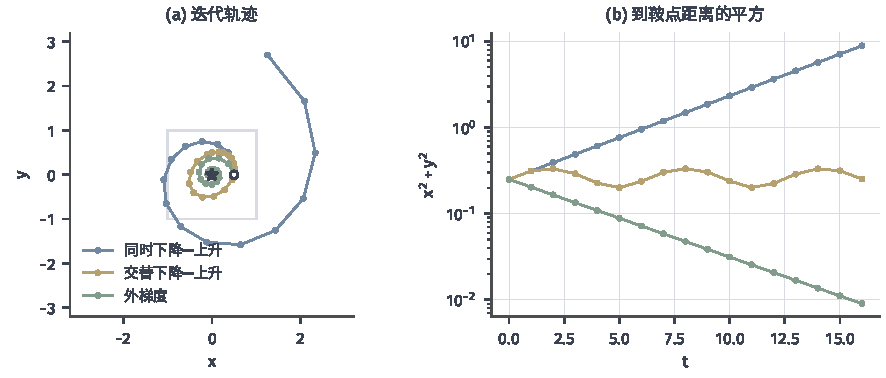
\includegraphics[width=150mm]{figures/03-optimization-evolution-and-signals/01-optimization/matplotlib/c7-gda-bilinear/figure.pdf}
  \caption{双线性目标$\phi(x,y)=xy$上的三种无约束迭代，步长$\eta=1/2$，起点$(1/2,0)$，共16步。(a)轨迹：同时下降—上升（蓝）向外螺旋，交替下降—上升（黄）在闭曲线附近打转，外梯度（绿）向内螺旋；灰框是盒$[-1,1]^2$，星号是鞍点。(b)到鞍点距离的平方（对数坐标）：蓝线每步乘$1+\eta^2=1.25$，绿线每步乘$1-\eta^2+\eta^4=0.8125$，黄线有界振荡。}
  \label{fig:opt-mmb-gda-bilinear}
\end{figure*}

\paragraph{加上投影也不收敛}
有界约束能阻止发散，却不能让迭代停到鞍点。在盒$X=Y=[-1,1]$上取$\eta=1$，从$(1,0)$出发执行算法~\ref{alg:opt-mmb-gda}：
\[
\begin{aligned}
&(1,0)\to(1,1)\to(0,1)\to(-1,1)\to(-1,0)\\
&\quad\to(-1,-1)\to(0,-1)\to(1,-1)\to(1,0).
\end{aligned}
\]
例如第一步$x^{(1)}=\Pi(1-0)=1$，$y^{(1)}=\Pi(0+1)=1$；第二步$x^{(2)}=\Pi(1-1)=0$，$y^{(2)}=\Pi(1+1)=1$。八步之后回到起点，间隙$|x|+|y|$在循环上始终不小于$1$，见图~\ref{fig:opt-mmb-box-cycle}。鞍点存在（定理~\ref{thm:opt-mmb-minimax}的条件全部满足），算法却不收敛：存在性定理回答的是“答案在不在”，不回答“这个算法能否找到它”。

\begin{figure}[!htbp]
  \centering
  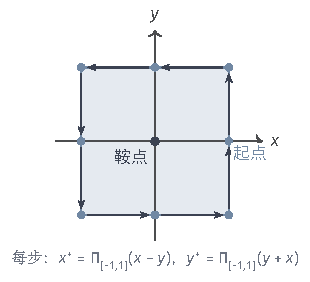
\includegraphics[width=52.5mm]{figures/03-optimization-evolution-and-signals/01-optimization/tikz/c7-box-cycle/figure.pdf}
  \caption{盒约束双线性问题上的投影同时梯度下降—上升，$\phi(x,y)=xy$，$X=Y=[-1,1]$，步长$\eta=1$。从$(1,0)$出发，迭代沿盒的四角与四边中点逆时针循环，周期为$8$；循环上的间隙$|x|+|y|$取$1$或$2$，永不趋于零。}
  \label{fig:opt-mmb-box-cycle}
\end{figure}

这个循环的八个点的平均恰好是原点，那是对称性的巧合。无约束的同时版本中，平均点$\frac1T\sum_{t<T}\bm u^{(t)}$的范数随$T$增大而趋于无穷，因为$\bm u^{(t)}$的范数以$(1+\eta^2)^{t/2}$的速度增长，平均也挽救不了。

\paragraph{用什么判断成功}
极小极大迭代是否成功，要看输出满足的是哪一种关系：可行性（投影后自动满足），间隙~\eqref{eq:opt-mmb-gap}，或者在凸凹且光滑时的投影残差$\lVert\bm u-\Pi_{X\times Y}(\bm u-\eta\bm F(\bm u))\rVert_2/\eta$（$\bm F$见下一小节）。单看某一方的目标是否下降没有意义。双线性例中，点$(0,y)$处$\phi=0$已经等于鞍点值，但它的间隙是$|y|$；最小化方的目标$\bar\phi(x)$可能在一段时间内下降，而最大化方此时正在变差。

\subsection{外梯度法}
\label{sec:opt-mmb-extragradient}

梯度下降—上升的问题在于，它用旧点的方向走一整步，而旋转向量场在一步之内就已经转向。外梯度法先试探性地走一步，看看那里的方向，再回到旧点按试探点的方向走。

\paragraph{两次求值、两次投影}
把双方合成一个变量$\bm u=(\bm x,\bm y)\in K=X\times Y$，令
\begin{equation}
\label{eq:opt-mmb-monotone-field}
\bm F(\bm u)=\bigl(\nabla_{\bm x}\phi(\bm x,\bm y),\ -\nabla_{\bm y}\phi(\bm x,\bm y)\bigr),
\end{equation}
则同时梯度下降—上升就是$\bm u^{(t+1)}=\Pi_K(\bm u^{(t)}-\eta\bm F(\bm u^{(t)}))$。\term{外梯度法}（extragradient method）\cite{korpelevich1976}每轮做两步：
\begin{equation}
\label{eq:opt-mmb-extragradient}
\bar{\bm u}^{(t)}=\Pi_K\bigl(\bm u^{(t)}-\eta\bm F(\bm u^{(t)})\bigr),\qquad
\bm u^{(t+1)}=\Pi_K\bigl(\bm u^{(t)}-\eta\bm F(\bar{\bm u}^{(t)})\bigr).
\end{equation}
第二步的起点仍是旧点$\bm u^{(t)}$，只是方向换成了试探点$\bar{\bm u}^{(t)}$处的方向。这与连续做两次普通梯度步不同：后者的第二步从$\bar{\bm u}^{(t)}$出发。每轮需要两次方向求值（各含一次$\nabla_{\bm x}\phi$与$\nabla_{\bm y}\phi$）和两次投影，返回$\bm u^{(t+1)}$，下面的平均保证则作用于试探点的平均。

\paragraph{双线性例中的校正}
仍取$\phi(x,y)=xy$，$\bm F(x,y)=(y,-x)$。图~\ref{fig:opt-mmb-extragradient-step}取旧点$\bm u=(1.6,0)$与$\eta=1/2$：$\bm F(\bm u)=(0,-1.6)$，试探点$\bar{\bm u}=(1.6,0.8)$；$\bm F(\bar{\bm u})=(0.8,-1.6)$，从旧点出发的校正点为$\bm u^+=(1.6-0.4,\,0+0.8)=(1.2,0.8)$，到鞍点的距离从$1.6$降到$\sqrt{2.08}\approx1.44$。若从试探点再走一次普通步，会到达$(1.2,1.6)$，距离增到$2$。试探点的方向已经“转过了一点”，用它从旧点出发，正好抵消了旋转造成的外漂。

\begin{figure}[!htbp]
  \centering
  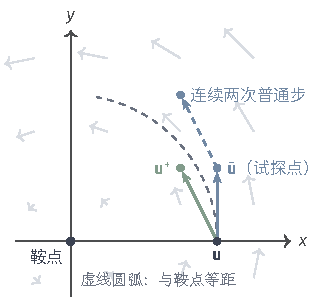
\includegraphics[width=54.0mm]{figures/03-optimization-evolution-and-signals/01-optimization/tikz/c7-extragradient-step/figure.pdf}
  \caption{外梯度法的一步，$\phi(x,y)=xy$，$\eta=1/2$。灰色短箭头是更新方向场$-\bm F=(-y,x)$，绕鞍点旋转。从旧点$\bm u=(1.6,0)$出发，普通步到达试探点$\bar{\bm u}=(1.6,0.8)$，若再走一次普通步（蓝色虚线）会到$(1.2,1.6)$；外梯度从$\bm u$出发、沿$\bar{\bm u}$处的方向走，得到$\bm u^+=(1.2,0.8)$（绿色），落在过$\bm u$的等距圆弧以内。}
  \label{fig:opt-mmb-extragradient-step}
\end{figure}

一般地，无约束时把式~\eqref{eq:opt-mmb-extragradient}代入$\bm F(x,y)=(y,-x)$得
\[
\bm u^{(t+1)}=\begin{pmatrix}1-\eta^2&-\eta\\ \eta&1-\eta^2\end{pmatrix}\bm u^{(t)},\qquad
\lVert\bm u^{(t+1)}\rVert_2^2=(1-\eta^2+\eta^4)\lVert\bm u^{(t)}\rVert_2^2,
\]
当$0<\eta<1$时因子小于$1$，距离几何收缩。回到盒约束，取$\eta=1/2$与$\lVert\bm u^{(0)}\rVert_2\leq1/2$：试探点的范数是$\sqrt{1+\eta^2}\,\lVert\bm u^{(t)}\rVert_2\leq\frac{\sqrt5}{4}<1$，校正点的范数不超过旧点，于是由归纳法所有点都留在单位圆盘内，而单位圆盘含于盒中，两次投影都不起作用。所以在这组初值和步长下，外梯度迭代以因子$\sqrt{13/16}$收敛到鞍点，间隙趋于零；同样的设置下，同时梯度下降—上升会离开盒子并在投影后进入图~\ref{fig:opt-mmb-box-cycle}那样的循环。

\paragraph{凸凹问题上的平均间隙保证}
双线性例的收缩依赖具体的矩阵。一般凸凹问题上，外梯度法的保证来自$\bm F$的两个性质。若$\phi$对$\bm x$凸、对$\bm y$凹且可微，则$\bm F$是单调的：$\langle\bm F(\bm u)-\bm F(\bm v),\bm u-\bm v\rangle\geq0$。此外假设$\bm F$在$K$上是$L$-Lipschitz的。

\begin{theorem}[外梯度法的平均间隙]
\label{thm:opt-mmb-extragradient}
设$X,Y$非空紧凸，$\phi$在包含$X\times Y$的开集上可微，对$\bm x$凸、对$\bm y$凹，$\bm F$在$K$上$L$-Lipschitz，$0<\eta\leq1/L$。记试探点$\bar{\bm u}^{(t)}=(\bar{\bm x}^{(t)},\bar{\bm y}^{(t)})$的平均为$(\hat{\bm x}_T,\hat{\bm y}_T)=\frac1T\sum_{t=0}^{T-1}\bar{\bm u}^{(t)}$，$K$的直径为$D_K$。则
\[
\operatorname{gap}(\hat{\bm x}_T,\hat{\bm y}_T)\leq\frac{D_K^2}{2\eta T}.
\]
\end{theorem}

\begin{proof}
投影的刻画可以写成：若$\bm p=\Pi_K(\bm z)$，则对任意$\bm v\in K$有$\lVert\bm p-\bm v\rVert_2^2\leq\lVert\bm z-\bm v\rVert_2^2-\lVert\bm z-\bm p\rVert_2^2$。固定$\bm v\in K$，省略迭代上标，记$\bm u,\bar{\bm u},\bm u^+$为一轮中的三个点。

对校正步用上式，展开平方得
\[
2\eta\langle\bm F(\bar{\bm u}),\bm u^+-\bm v\rangle\leq\lVert\bm u-\bm v\rVert_2^2-\lVert\bm u^+-\bm v\rVert_2^2-\lVert\bm u-\bm u^+\rVert_2^2.
\]
对试探步用投影刻画$\langle\bm u-\eta\bm F(\bm u)-\bar{\bm u},\bm u^+-\bar{\bm u}\rangle\leq0$，并用恒等式$2\langle\bm a-\bm b,\bm b-\bm c\rangle=\lVert\bm a-\bm c\rVert_2^2-\lVert\bm a-\bm b\rVert_2^2-\lVert\bm b-\bm c\rVert_2^2$，得
\[
2\eta\langle\bm F(\bm u),\bar{\bm u}-\bm u^+\rangle\leq\lVert\bm u-\bm u^+\rVert_2^2-\lVert\bm u-\bar{\bm u}\rVert_2^2-\lVert\bar{\bm u}-\bm u^+\rVert_2^2.
\]
由Lipschitz条件与$\eta L\leq1$，
\[
\begin{aligned}
2\eta\langle\bm F(\bar{\bm u})-\bm F(\bm u),\bar{\bm u}-\bm u^+\rangle&\leq2\eta L\lVert\bar{\bm u}-\bm u\rVert_2\lVert\bar{\bm u}-\bm u^+\rVert_2\\
&\leq\lVert\bar{\bm u}-\bm u\rVert_2^2+\lVert\bar{\bm u}-\bm u^+\rVert_2^2.
\end{aligned}
\]
把$2\eta\langle\bm F(\bar{\bm u}),\bar{\bm u}-\bm v\rangle$拆成上面三项之和，所有平方差相互抵消，得到
\[
2\eta\langle\bm F(\bar{\bm u}^{(t)}),\bar{\bm u}^{(t)}-\bm v\rangle\leq\lVert\bm u^{(t)}-\bm v\rVert_2^2-\lVert\bm u^{(t+1)}-\bm v\rVert_2^2.
\]
对$t=0,\dots,T-1$求和，右侧逐项相消，不超过$\lVert\bm u^{(0)}-\bm v\rVert_2^2\leq D_K^2$。

再把内积换成函数值。写$\bm v=(\bm x,\bm y)$。由$\phi(\cdot,\bar{\bm y}^{(t)})$凸与$\phi(\bar{\bm x}^{(t)},\cdot)$凹的一阶刻画，
\[
\langle\bm F(\bar{\bm u}^{(t)}),\bar{\bm u}^{(t)}-\bm v\rangle\geq\phi(\bar{\bm x}^{(t)},\bm y)-\phi(\bm x,\bar{\bm y}^{(t)}).
\]
对$t$平均，并再次用凸凹性（Jensen不等式）得$\phi(\hat{\bm x}_T,\bm y)-\phi(\bm x,\hat{\bm y}_T)\leq D_K^2/(2\eta T)$。左侧对$\bm y\in Y$取最大、对$\bm x\in X$取最小，即为$\operatorname{gap}(\hat{\bm x}_T,\hat{\bm y}_T)$。
\end{proof}

这一保证有三点需要分清。第一，它是关于平均点的间隙界，不是关于最后一个迭代点；在单调且Lipschitz、步长严格小于$1/L$的条件下，还可以证明外梯度的迭代点本身收敛到某个鞍点，但最后一点的间隙速率需要另作分析，不能直接沿用上面的平均点界。第二，证明用到的是凸凹性带来的单调性与Lipschitz连续性，而不是“多算了一次梯度”这一动作本身；在非凸非凹问题上，外梯度法同样可能循环或停在非鞍点的驻点。第三，同样的推导对同时梯度下降—上升走不通：没有试探点，上面第二、三个不等式无从得到，图~\ref{fig:opt-mmb-gda-bilinear}正是这一缺口的数值表现。

计算代价方面，外梯度每轮的方向求值和投影都是同时梯度下降—上升的两倍。比较两种方法时应按求值次数而不是轮数计费；若还要报告间隙，求$\bar\phi(\hat{\bm x}_T)$与$\underline\phi(\hat{\bm y}_T)$这两个最优响应问题的成本也要计入。
